\begin{figure}[H]
	\centering
	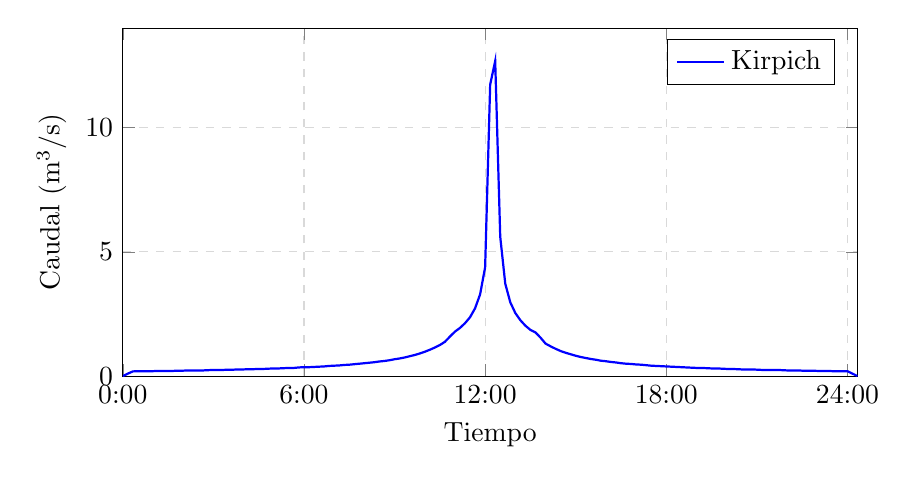
\begin{tikzpicture}
		\begin{axis}[
			width=0.9\textwidth,
			height=6cm,
			xlabel={Tiempo},
			ylabel={Caudal (m$^3$/s)},
			xmin=0,
			xmax=1460,
			ymin=0,
			ymax=14,
			grid=major,
			grid style={dashed, gray!30},
			legend pos=north east,
			xtick={0, 360, 720, 1080, 1440},
			xticklabels={0:00, 6:00, 12:00, 18:00, 24:00},
			]
		% Kirpich
		\addplot [
		blue,
		thick,
		solid,
		] coordinates {
				(0, 0.00) (10, 0.10) (20, 0.19) (30, 0.20) (40, 0.20)
				(50, 0.20) (60, 0.20) (70, 0.21) (80, 0.21) (90, 0.21)
				(100, 0.21) (110, 0.22) (120, 0.22) (130, 0.23) (140, 0.23)
				(150, 0.23) (160, 0.23) (170, 0.24) (180, 0.25) (190, 0.25)
				(200, 0.25) (210, 0.26) (220, 0.26) (230, 0.27) (240, 0.27)
				(250, 0.28) (260, 0.28) (270, 0.29) (280, 0.29) (290, 0.30)
				(300, 0.31) (310, 0.31) (320, 0.32) (330, 0.33) (340, 0.33)
				(350, 0.35) (360, 0.36) (370, 0.36) (380, 0.37) (390, 0.38)
				(400, 0.39) (410, 0.41) (420, 0.42) (430, 0.43) (440, 0.45)
				(450, 0.46) (460, 0.48) (470, 0.50) (480, 0.52) (490, 0.54)
				(500, 0.56) (510, 0.59) (520, 0.61) (530, 0.64) (540, 0.68)
				(550, 0.71) (560, 0.75) (570, 0.80) (580, 0.85) (590, 0.91)
				(600, 0.98) (610, 1.06) (620, 1.15) (630, 1.25) (640, 1.38)
				(650, 1.59) (660, 1.79) (670, 1.94) (680, 2.13) (690, 2.37)
				(700, 2.73) (710, 3.29) (720, 4.38) (730, 11.73) (740, 12.68)
				(750, 5.61) (760, 3.72) (770, 2.97) (780, 2.54) (790, 2.25)
				(800, 2.03) (810, 1.86) (820, 1.76) (830, 1.55) (840, 1.31)
				(850, 1.20) (860, 1.10) (870, 1.01) (880, 0.94) (890, 0.88)
				(900, 0.82) (910, 0.77) (920, 0.73) (930, 0.69) (940, 0.66)
				(950, 0.62) (960, 0.60) (970, 0.57) (980, 0.55) (990, 0.52)
				(1000, 0.50) (1010, 0.49) (1020, 0.47) (1030, 0.46) (1040, 0.44)
				(1050, 0.42) (1060, 0.41) (1070, 0.40) (1080, 0.39) (1090, 0.38)
				(1100, 0.37) (1110, 0.36) (1120, 0.35) (1130, 0.34) (1140, 0.33)
				(1150, 0.33) (1160, 0.32) (1170, 0.31) (1180, 0.31) (1190, 0.30)
				(1200, 0.29) (1210, 0.29) (1220, 0.28) (1230, 0.27) (1240, 0.27)
				(1250, 0.27) (1260, 0.26) (1270, 0.25) (1280, 0.25) (1290, 0.25)
				(1300, 0.25) (1310, 0.24) (1320, 0.23) (1330, 0.23) (1340, 0.23)
				(1350, 0.22) (1360, 0.22) (1370, 0.22) (1380, 0.21) (1390, 0.21)
				(1400, 0.21) (1410, 0.20) (1420, 0.20) (1430, 0.20) (1440, 0.20)
				(1450, 0.10) (1460, 0.00)
		};
		\addlegendentry{Kirpich}

		\end{axis}
	\end{tikzpicture}
	\caption{Hidrograma - Kirpich + BLOCKS24 $T_r$=25 años ($Q_p$=12.679 m$^3$/s)}
	\label{fig:hydro_kirpich_blocks24_Tr25}
\end{figure}
